\documentclass[12pt,a4paper]{article}

% =============================
% PACKAGES
% =============================
\usepackage[a4paper,margin=1in]{geometry}
\usepackage{lmodern}
\usepackage[T1]{fontenc}
\usepackage[utf8]{inputenc}
\usepackage{microtype}
\usepackage{titlesec}
\usepackage{booktabs}
\usepackage{array}
\usepackage{graphicx}
\usepackage{caption}
\usepackage{subcaption}
\usepackage{amsmath}
\usepackage{amssymb}
\usepackage[hidelinks,colorlinks=true,linkcolor=primaryblue,citecolor=primaryblue,urlcolor=primaryblue]{hyperref}
\hypersetup{
  pdftitle={Modelling Sinusoidal Pressure-Driven Micro-Scale Flow in a Water-Based Star Microchannel},
  pdfauthor={Dhruv Upadhyay, Saket Kumar Singh, Sudarshan Kumar Oraon, Yugal Kishore Misra},
  pdfsubject={Microfluidics and Microfabrication},
  pdfkeywords={Microfluidics, Pulsatile Flow, COMSOL, Star Microchannel, Navier-Stokes}
}
\usepackage{enumitem}
\usepackage{setspace}
\usepackage{xcolor}
\usepackage{tabularx}
\usepackage{multirow}
\usepackage{float}

% =============================
% COLOR DEFINITIONS
% =============================
\definecolor{primaryblue}{RGB}{0,71,171}
\definecolor{secondaryblue}{RGB}{41,128,185}
\definecolor{lightgray}{RGB}{245,245,245}
\definecolor{darkgray}{RGB}{100,100,100}

% =============================
% STYLE SETTINGS
% =============================
\setstretch{1.15}
\setlength{\parskip}{8pt plus 3pt minus 2pt}
\setlength{\parindent}{0pt}
\setlist[itemize]{leftmargin=2em,topsep=6pt,itemsep=4pt,parsep=2pt}
\setlist[enumerate]{leftmargin=2em,topsep=6pt,itemsep=4pt,parsep=2pt}

% Section formatting with enhanced academic style
\titleformat{\section}
  {\Large\bfseries\color{primaryblue}}{\thesection.}{0.8em}{\MakeUppercase}
  [\vspace{-4pt}{\color{primaryblue}\titlerule[1.5pt]}\vspace{10pt}]
\titleformat{\subsection}
  {\large\bfseries\color{secondaryblue}}{\thesubsection}{0.6em}{}
  [\vspace{3pt}]
\titleformat{\subsubsection}
  {\normalsize\bfseries\itshape\color{secondaryblue}}{\thesubsubsection}{0.5em}{}

\titlespacing*{\section}{0pt}{12pt plus 2pt minus 1pt}{6pt plus 1pt minus 1pt}
\titlespacing*{\subsection}{0pt}{8pt plus 2pt minus 1pt}{4pt plus 1pt minus 1pt}
\titlespacing*{\subsubsection}{0pt}{6pt plus 1pt minus 1pt}{3pt plus 1pt minus 1pt}

\renewcommand{\arraystretch}{1.2}

% Table of Contents formatting with professional appearance
\usepackage{titletoc}
\titlecontents{section}[1.5em]
  {\vspace{0.7em}\bfseries\color{primaryblue}}
  {\contentslabel{1.5em}}
  {\hspace*{-1.5em}}
  {\titlerule*[0.8pc]{.}\contentspage}
\titlecontents{subsection}[3.8em]
  {\vspace{0.3em}\color{darkgray}}
  {\contentslabel{2.3em}}
  {\hspace*{-2.3em}}
  {\titlerule*[0.8pc]{.}\contentspage}

% Header and Footer
\usepackage{fancyhdr}
\pagestyle{fancy}
\fancyhf{}
\lhead{\color{primaryblue}\small\textit{CLL770: Microfluidics \& Microfabrication}}
\rhead{\color{primaryblue}\small Page \thepage}
\renewcommand{\headrulewidth}{0.4pt}
\renewcommand{\headrule}{\hbox to\headwidth{\color{primaryblue}\leaders\hrule height \headrulewidth\hfill}}
\setlength{\headheight}{24.02pt}

% Caption styling with better spacing
\captionsetup{
  font=small,
  labelfont={bf,color=primaryblue},
  textfont=it,
  skip=10pt,
  position=below
}

% =============================
% CUSTOM COMMANDS
% =============================
\newcommand{\authorinfo}[2]{%
  \textbf{#1} \\
  \textit{Entry No:} #2 \\[0.3em]
}

% =============================
% DOCUMENT START
% =============================
\begin{document}

% =============================
% TITLE PAGE
% =============================
\begin{titlepage}
  \centering
  \vspace*{1cm}
  
  % University Logo
  
\includegraphics[width=0.35\textwidth]{images/image.png}
  
  \vspace{0.8cm}
  
{\LARGE\bfseries\color{primaryblue} INDIAN INSTITUTE OF TECHNOLOGY}\\[0.8em]
{\LARGE\bfseries\color{primaryblue}\textls[80]{DELHI}}\\[0.2em]
  {\large\color{secondaryblue} Department of Chemical Engineering}\\[2.5cm]
  
  % Course Code Box
  \fcolorbox{primaryblue}{lightgray!20}{%
    \parbox{0.7\textwidth}{%
      \centering
      \vspace{0.4cm}
      {\Large\bfseries\color{primaryblue} CLL770}\\[0.4em]
      {\large\color{secondaryblue}\textsc{Introduction to Microfluidics and Microfabrication}}\\
      \vspace{0.4cm}
    }
  }
  
  \vspace{2cm}
  
  % Report Title
  {\huge\bfseries\color{primaryblue} 
  Modelling Sinusoidal Pressure--Driven\\[0.4em]
  Micro-Scale Flow in a Water-Based\\[0.4em]
  Star Microchannel}\\[2.5cm]
  
  % Authors Section
  \begin{minipage}{0.85\textwidth}
    \begin{center}
      {\Large\bfseries\color{secondaryblue} PROJECT REPORT}\\[1.2cm]
      
      \renewcommand{\arraystretch}{1.3}
      \begin{tabular}{>{\raggedright}p{0.5\textwidth}l}
        \multicolumn{2}{c}{\Large\bfseries\color{primaryblue} Authors} \\[0.6em]
        \toprule
        \textbf{Name} & \textbf{Entry Number} \\
        \midrule
        Dhruv Upadhyay & 2022CH71484 \\
        Saket Kumar Singh & 2022CH71478 \\
        Sudarshan Kumar Oraon & 2022CH71511 \\
        Yugal Kishore Misra & 2022CH71039 \\
        \bottomrule
      \end{tabular}
    \end{center}
  \end{minipage}
  
  \vfill
  
  {\large Submission Date: 19 November 2025}
  
\end{titlepage}

\pagestyle{fancy}

% =============================
% ACKNOWLEDGEMENTS
% =============================
\newpage
\section*{Acknowledgements}
\addcontentsline{toc}{section}{Acknowledgements}

\vspace{0.5cm}

\noindent We would like to express our sincere gratitude to \textbf{Professor Mohan Kumar Singh Verma}, Department of Chemical Engineering, IIT Delhi, for his invaluable guidance, continuous encouragement, and expert insights throughout this research project. His profound knowledge in the field of microfluidics and microfabrication has been instrumental in shaping the direction and depth of this study. This work would not have been possible without his mentorship and support.

\vspace{0.5cm}

% =============================
% PEER EVALUATION
% =============================
\section*{Peer Evaluation}
\addcontentsline{toc}{section}{Peer Evaluation}

\noindent Please evaluate your team members based on their contribution to the group:
\begin{itemize}
  \item 5 = This team member made unique and irreplaceable contributions to the group
  \item 4 = This team member made important contributions to the group
  \item 3 = This team member made a satisfactory contribution to the group
  \item 2 = This team member made a sub-par contribution to the group
  \item 1 = This team member was frequently absent and contributed very little to the group
  \item 0 = This team member was completely absent or disruptive to the group
\end{itemize}

\vspace{1em}

\begin{table}[h]
\centering
\begin{tabular}{clcc}
\toprule
\textbf{S.No.} & \textbf{Team Member Name} & \textbf{Entry Number} & \textbf{Ranking} \\
\midrule
1 & Dhruv Upadhyay & 2022CH71484 & 5 \\
2 & Saket Kumar Singh & 2022CH71478 & 5 \\
3 & Sudarshan Kumar Oraon & 2022CH71511 & 5 \\
4 & Yugal Kishore Misra & 2022CH71039 & 5 \\
\bottomrule
\end{tabular}
\end{table}

% =============================
% ABSTRACT
% =============================
\newpage
\section*{Abstract}
\addcontentsline{toc}{section}{Abstract}

\vspace{0.5cm}

\noindent\fcolorbox{primaryblue}{lightgray!10}{%
  \parbox{0.96\textwidth}{%
    \vspace{0.6cm}
    \setlength{\parskip}{10pt}
    \noindent\textbf{Background and Motivation:} This study presents a comprehensive computational investigation of pulsatile microfluidic flow in a star-shaped 5-inlet converging channel, representing a synthetic venule (microvascular drainage network). The channel geometry is modeled in COMSOL Multiphysics as a three-dimensional laminar flow domain. Each of the five inlets is driven by a sinusoidal pressure boundary condition with equal amplitude but staggered phase shifts, while the outlet is held at reference pressure. Time-dependent incompressible Navier--Stokes equations (Laminar Flow interface) are solved for a water-like fluid. 

    \noindent\textbf{Results and Findings:} The simulation results demonstrate that at any given instant, the inlet exhibiting the highest pressure (designated as the ``active inlet'') dominates the flow dynamics, generating a high-velocity jet directed toward the common outlet and establishing a rotating high-pressure zone around the star geometry throughout the pulsation cycle. Velocity field analysis and particle trajectory visualization confirm that fluid from all inlet branches converges toward the outlet, with the jet position sweeping cyclically in correspondence with the phase-shifted driving conditions. Parametric sensitivity analysis reveals that increasing the pressure amplitude proportionally scales the flow magnitude, whereas increasing the pulsation frequency compresses the temporal oscillation period without affecting peak velocity magnitudes.
    
    \noindent\textbf{Significance:} These findings demonstrate that multi-inlet pulsatile driving strategies can generate nearly continuous net outflow while dynamically reconfiguring internal flow paths---a phenomenon analogous to the physiological drainage of capillaries into venules. The results have direct implications for the design of biomimetic microfluidic systems and organ-on-chip platforms.
    \vspace{0.6cm}
  }%
}

\vspace{1em}

% =============================
% TABLE OF CONTENTS
% =============================
\newpage
\tableofcontents
\newpage

% =============================
% MAIN CONTENT
% =============================

\section{Introduction}

Microfluidic systems typically operate in the low-Reynolds-number (laminar) regime, where fluid mixing and flow control mechanisms must be achieved through strategic design of time-varying inputs or specialized geometric configurations. In biological systems, microcirculation is characterized by inherently pulsatile pressure waves originating from cardiac cycles, which propagate through extensive capillary networks. Despite this physiological reality, the majority of laboratory-based lab-on-a-chip models employ steady-state or simple time-invariant flow conditions for the sake of experimental simplicity. 

A comprehensive understanding of pulsatile microscale flow dynamics is crucial for advancing applications in targeted drug delivery, nutrient transport modeling, and disease pathology studies at the capillary level. The complex interplay between temporal pressure variations and microscale geometries remains an underexplored area in microfluidic research, particularly in the context of multi-inlet drainage networks. 

In the physiological microvasculature, numerous capillaries converge into collecting venules, forming complex drainage networks. However, current organ-on-chip (OoC) research predominantly focuses on arterial/perfusion dynamics while the pulsatile outflow behavior on the venous drainage side remains relatively unexplored. To address this gap, we have developed a \textit{synthetic venule model} consisting of a star-shaped microchannel architecture with five inlet branches that merge into a single outlet channel. Through the application of phase-shifted sinusoidal pressure boundary conditions at each inlet, we systematically emulate the asynchronous pulsatile dynamics characteristic of converging capillary networks.

\begin{figure}[H]
  \centering
  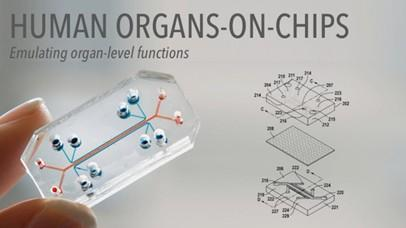
\includegraphics[width=0.75\textwidth]{images/1.png}
  \caption{Major types of blood vessels showing arteries, veins, and capillaries in biological circulatory systems.}
  \label{fig:blood_vessels}
\end{figure}

Numerical simulation (using COMSOL Multiphysics) allows detailed visualization of the unsteady flow fields, which would be difficult to measure experimentally at this scale. Time-dependent finite-element analysis solves the incompressible Navier--Stokes equations in 3D, generating velocity and pressure fields throughout the cycle. We examine how the instantaneous dominant inlet changes over time, how the flow jets reorient, and how the pressure distributes across the network. Sensitivity to driving amplitude and frequency is also assessed. Finally, we interpret these results in the context of microvascular drainage (e.g., nearly continuous venular flow despite upstream pulsatility) and microfluidic mixing (e.g., dynamic sweeping of interfaces).

\subsection{Organization of This Report}

This research report is organized according to standard academic conventions:
\begin{enumerate}
  \item \textbf{Motivation}: Articulation of the scientific rationale and practical significance of investigating pulsatile drainage dynamics in synthetic venule geometries
  \item \textbf{Methodology}: Comprehensive description of the computational framework, including geometric design, governing equations, boundary conditions, and numerical implementation in COMSOL Multiphysics
  \item \textbf{Results}: Systematic presentation of simulation outcomes, including temporal velocity and pressure field evolution, parametric sensitivity analysis, and particle trajectory visualization
  \item \textbf{Discussion}: Critical interpretation of results in the context of microvascular physiology and microfluidic applications, with explicit treatment of model assumptions and limitations
  \item \textbf{Future Work}: Identification of promising research directions for model refinement and experimental validation
  \item \textbf{Conclusion}: Summary of principal findings and their implications for microfluidic device design and biomimetic systems
\end{enumerate}

\section{Motivation}

The motivation for this computational study encompasses two interconnected research objectives: (i) developing accurate models of microvascular drainage dynamics, and (ii) advancing the understanding of microfluidic mixing phenomena and organ-on-chip outflow behavior under physiologically relevant pulsatile conditions.

\subsection{Microvascular Drainage Modeling}

In physiological systems, capillary beds serve as drainage networks that converge into collecting venules, wherein multiple small-diameter vessels channel fluid into a single downstream conduit. While the arterial (perfusion) side of microcirculation has received substantial research attention, the pulsatile flow dynamics governing venous drainage remain comparatively understudied despite their critical importance for maintaining proper tissue perfusion and metabolic homeostasis. By constructing a synthetic \textit{venule} analog---a star-shaped microchannel where five small branches merge---we can study how pulsatile inputs interact and produce net outflow. Notably, if the inlets are phased, their oscillations can partially cancel, leading to a smoother net flow (a form of physiological ``flow moderation'').

\subsection{Microfluidic Mixing and Organ-on-Chip Applications}

In contemporary microfluidic applications---including microscale reactors, mixing devices, and organ-on-chip platforms---a thorough understanding of unsteady convergence flow phenomena is essential for optimal system design. While laboratory investigations frequently employ steady-state flow conditions to reduce experimental complexity, authentic physiological flows exhibit inherent pulsatility. For instance, tissue-on-chip devices require faithful representation of both tissue perfusion (inflow) and metabolic drainage (outflow) processes. In such systems, multiple waste or effluent streams converge, and strategic implementation of time-varying actuation protocols may significantly enhance mixing efficiency and metabolite transport kinetics. 

Existing COMSOL examples demonstrate pulsatile flows in simple geometries, but seldom do they tackle a network with multiple converging pulsatile sources. This gap is significant: asynchronous pulses from different inlets could lead to novel flow patterns (e.g., rotating jets) that neither steady nor single-inlet pulsatile models capture.

Thus, by modeling a five-inlet pulsatile microchannel, we aim to show:
\begin{enumerate}[label=(\alph*)]
  \item How inlet dominance rotates over time
  \item How pressure gradients are established
  \item How the combined outflow behaves
  \item How system response scales with pumping parameters
\end{enumerate}

These insights can inform the design of microfluidic OoC drainage networks and microreactors. As a bonus, the model provides an easily replicable demonstration of pulsatile multi-inlet flows for educational purposes (e.g., illustrating phase-shift effects).

\newpage
\section{Methodology}

\subsection{Computational Domain and Mesh Generation}

The computational domain consists of a three-dimensional star-shaped microchannel geometry comprising five inlet branches arranged in symmetric radial configuration around a central drainage channel. Each inlet branch is modeled as a straight conduit with rectangular cross-section, with characteristic dimensions (width and height) on the order of 50--200~$\mu$m to faithfully represent capillary-scale flow conditions. These branches converge into a common main channel that terminates at a single outlet boundary.

The geometric design draws inspiration from the COMSOL Multiphysics ``Star-Shaped Microchannel'' benchmark model, with dimensional parameters specifically selected to emulate physiological capillary networks. All channel walls are treated as rigid boundaries with no-slip conditions imposed to accurately capture near-wall velocity gradients.

\begin{figure}[H]
  \centering
    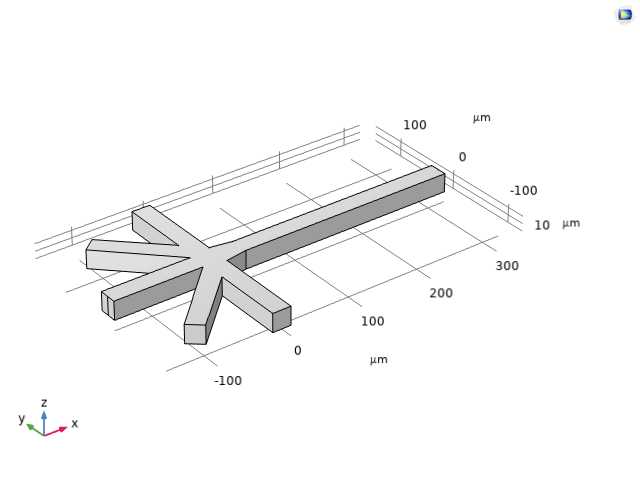
\includegraphics[width=0.6\textwidth]{images/2.png}
  \caption{Schematic representation of the star-shaped microchannel geometry with five inlet branches converging into a single outlet.}
  \label{fig:geometry}
\end{figure}

\subsubsection{Mesh Strategy}

A structured finite-element mesh was generated utilizing an extruded prismatic element topology, featuring high aspect ratio elements oriented along the principal flow direction to efficiently capture streamwise velocity gradients while minimizing computational overhead. Strategic mesh refinement was implemented in regions of geometric complexity, particularly near inlet junction zones, to ensure accurate resolution of local flow features including recirculation zones and pressure gradients.

The temporal discretization scheme employed a time-dependent solver with adaptive time-stepping, maintaining temporal resolution on the order of milliseconds to adequately resolve the imposed sinusoidal pressure waveforms throughout complete pulsation cycles.

\subsection{Governing Equations and Fluid Properties}

The flow physics are governed by the incompressible Navier--Stokes equations, comprising the continuity equation (mass conservation) and momentum conservation equations for laminar, single-phase flow. The working fluid is modeled as water at standard ambient conditions (298~K, 1~atm) with the following thermophysical properties:
\begin{itemize}
  \item Density: $\rho = 998$ kg/m³
  \item Dynamic viscosity: $\mu = 1.002 \times 10^{-3}$ Pa·s
  \item Kinematic viscosity: $\nu = \mu/\rho \approx 1.004 \times 10^{-6}$ m²/s
\end{itemize}

This Newtonian fluid approximation provides a well-defined baseline for investigating fundamental hydrodynamic behavior while avoiding the complexities associated with non-Newtonian rheology, particulate suspensions, or cellular constituents. Although blood exhibits shear-thinning viscoelastic behavior, the simplified model captures essential flow physics and can be readily extended to incorporate more sophisticated constitutive relations in future work. Body forces (gravity) are neglected given the microscale dimensions and low Bond number.

The governing equations, derived for single-phase, incompressible flow, are expressed in tensor notation as follows:

\textbf{Continuity equation:}
\begin{equation}
\nabla \cdot \mathbf{u} = 0
\end{equation}

\textbf{Momentum equation:}
\begin{equation}
\rho \left( \frac{\partial \mathbf{u}}{\partial t} + \mathbf{u} \cdot \nabla \mathbf{u} \right) = -\nabla p + \mu \nabla^2 \mathbf{u}
\end{equation}

where $\mathbf{u}$ is the velocity vector, $p$ is pressure, $\rho$ is density, and $\mu$ is dynamic viscosity.

% \begin{figure}[H]
%   \centering
%   \fcolorbox{primaryblue}{lightgray!30}{%
%     \parbox{0.75\textwidth}{%
%       \centering
%       \vspace{2.5cm}
%       \textcolor{primaryblue}{\large\textbf{[Image Placeholder]}}\\[0.5em]
%       \textcolor{darkgray}{\textit{Governing equations diagram}}\\
%       \textcolor{darkgray}{\small Visual representation of Navier-Stokes equations}
%       \vspace{2.5cm}
%     }
%   }
%   \caption{Governing equations for incompressible Navier--Stokes flow in tensor notation.}
%   \label{fig:equations}
% \end{figure}

\section{Boundary Conditions}

The specification of physically realistic and mathematically well-posed boundary conditions is essential for accurate simulation of pulsatile microscale flow within the star-shaped microchannel geometry. The following boundary conditions were implemented in the COMSOL Multiphysics finite-element framework.

\subsection{Wall Boundary Conditions}

All solid-fluid interfaces (channel walls) were assigned the standard \textbf{no-slip boundary condition}, mathematically expressed as:
\begin{equation}
\mathbf{u}|_{\text{wall}} = \mathbf{0}
\end{equation}
This condition ensures zero tangential and normal velocity components at all wall surfaces, consistent with the continuum hypothesis and validated by extensive experimental observations in microfluidic systems. The no-slip assumption is particularly appropriate in the low-Reynolds-number regime characteristic of microscale flows, where viscous forces dominate over inertial effects and molecular-level wall interactions strongly influence near-wall velocity profiles.

\subsection{Inlet Boundary Conditions}

Each of the five inlet boundaries was prescribed a \textbf{time-dependent sinusoidal pressure waveform} to emulate physiological pulsatility. The pressure at inlet $i$ is mathematically expressed as:

\begin{equation}
P_i(t) = P_0 + A \sin(\omega t + \phi_i), \quad i = 1, 2, \ldots, 5
\label{eq:inlet_pressure}
\end{equation}

where the parameters are defined as follows:
\begin{itemize}
  \item $P_0$ --- baseline (mean) pressure [Pa]
  \item $A$ --- pressure oscillation amplitude [Pa]
  \item $\omega = 2\pi f$ --- angular frequency of pulsation [rad/s]
  \item $f$ --- frequency [Hz]
  \item $\phi_i$ --- phase offset for inlet $i$ [rad]
\end{itemize}

The phase offsets $\phi_i$ were systematically varied to create asynchronous pressure waves at different inlets, with phase shifts of $\Delta\phi = 2\pi/5$ radians (72$^\circ$) between consecutive inlets. This phase-shifting strategy generates a temporally rotating pattern of inlet dominance, thereby mimicking the physiological scenario wherein pressure waves propagate through branching capillary networks with characteristic time delays arising from wave propagation and compliance effects.

\subsection{Outlet Boundary Conditions}

The single outlet was maintained at a \textbf{constant (reference) pressure}, enabling fluid to drain freely from the microchannel. A smooth pressure gradient from the inlets toward the outlet ensures physically realistic unidirectional flow.

\subsection{Initial Conditions}

The simulation was initialized using a \textbf{quiescent fluid} condition (zero initial velocity). This allows the sinusoidal pressure wave to fully drive the subsequent transient flow field.

\section{Results}

This section presents the principal outcomes of the computational simulations, highlighting the complex spatiotemporal flow dynamics induced by phase-shifted sinusoidal pressure boundary conditions. Results are organized to systematically demonstrate velocity field evolution, pressure distribution patterns, and parametric sensitivity.

\subsection{Temporal Evolution of the Velocity Field}

Figure~\ref{fig:velocity_field} presents representative velocity magnitude contours at selected time instants throughout a complete pulsation cycle. The simulation results reveal that at any given instant, the inlet experiencing the maximum instantaneous pressure (the ``active'' inlet) generates the most pronounced velocity jet directed toward the central outlet. High-velocity regions (depicted in red, $|\mathbf{u}| > 0.01$ m/s) sweep systematically across the microchannel junction as inlet dominance rotates in accordance with the imposed phase shifts. Correspondingly, low-velocity zones (blue, $|\mathbf{u}| < 0.001$ m/s) migrate in a complementary fashion, establishing dynamic recirculation patterns.

These observations confirm that phase-shifted pulsatile inlet conditions can effectively reorganize internal flow pathlines on time scales comparable to the pulsation period, a phenomenon with significant implications for microfluidic mixing and particle manipulation strategies.

\begin{figure}[H]
  \centering
  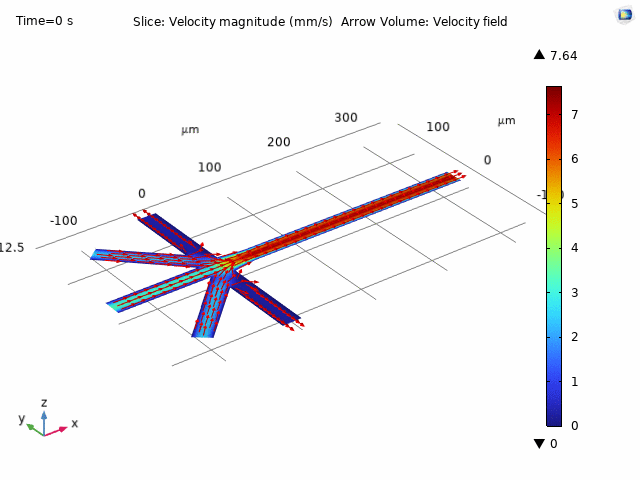
\includegraphics[width=0.85\textwidth]{images/3.png}
  \caption{Time-dependent velocity field showing the rotating high-velocity jet pattern as inlet dominance shifts. Red regions indicate high velocity; blue regions indicate low velocity.}
  \label{fig:velocity_field}
\end{figure}

\subsection{Temporal Evolution of Pressure Distribution}

Figure~\ref{fig:pressure_field} illustrates the spatial distribution of pressure at multiple time instants, revealing a systematically rotating high-pressure zone within the star-shaped junction region. At each temporal snapshot, the inlet experiencing peak sinusoidal pressure manifests as a localized high-pressure region (red contours), while the pressure field exhibits smooth monotonic decay along the central drainage channel toward the outlet boundary (maintained at reference pressure $P_0$).

The temporal sequence confirms that pressure waves propagate through the microscale network in accordance with the imposed phase relationships, establishing instantaneous pressure gradients that drive the observed velocity distributions. The absence of pressure discontinuities or numerical artifacts validates the computational solution and confirms adherence to fundamental mass conservation principles.

\begin{figure}[H]
  \centering
    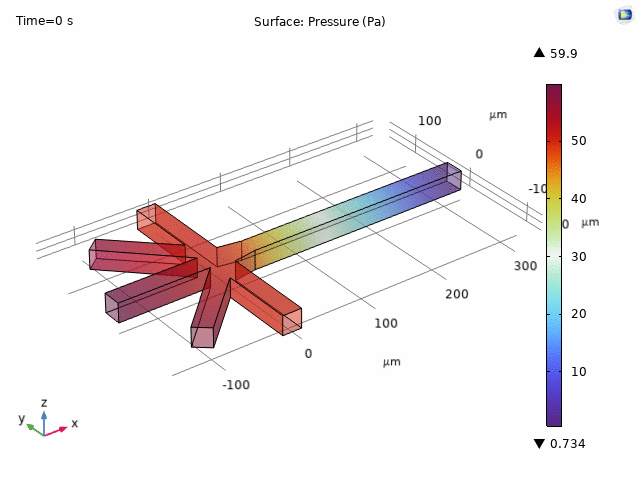
\includegraphics[width=0.85\textwidth]{images/4.png}
  \caption{Time-dependent pressure distribution showing rotating high-pressure zones corresponding to the active inlet at each time instant.}
  \label{fig:pressure_field}
\end{figure}

\subsection{Temporal Pressure Waveforms}

Figure~\ref{fig:pressure_time} presents the temporal evolution of inlet pressure for all five branches over multiple pulsation cycles. The plot confirms that each inlet exhibits ideal sinusoidal time-dependence with prescribed amplitude $A$ and frequency $f$, with successive inlets phase-shifted by $\Delta\phi = 72^\circ$ (corresponding to $2\pi/5$ radians). The staggered peak occurrences validate correct implementation of the time-dependent boundary conditions (Eq.~\ref{eq:inlet_pressure}) and clearly illustrate the periodic rotation of inlet dominance. The periodic steady state is achieved after approximately two cycles, beyond which the solution exhibits perfect temporal periodicity.

\begin{figure}[H]
  \centering
  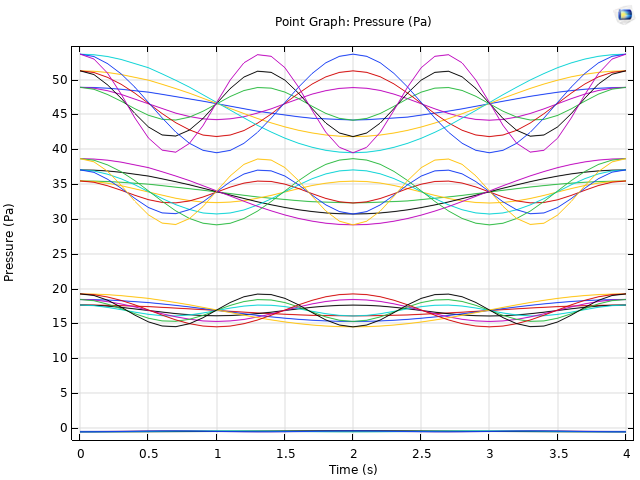
\includegraphics[width=0.85\textwidth]{images/5.png}
  \caption{Pressure vs time for all five inlets showing phase-shifted sinusoidal waveforms. Each curve represents a different inlet with staggered peaks.}
  \label{fig:pressure_time}
\end{figure}

\subsection{Parametric Sensitivity: Pressure Amplitude}

Figure~\ref{fig:velocity_amplitude} presents the results of a parametric sensitivity study wherein the pressure amplitude $A$ was systematically varied while maintaining constant frequency and phase relationships. Analysis of the velocity magnitude at a representative monitoring point (located at the junction center) as a function of time reveals two key findings:

\begin{enumerate}
  \item \textbf{Linear scaling}: Peak velocity magnitude scales linearly with pressure amplitude, indicating that $u_{\text{max}} \propto A$. This behavior is consistent with the dominance of viscous forces in the low-Reynolds-number regime.
  \item \textbf{Frequency invariance}: The temporal frequency of velocity oscillations remains unchanged across all amplitude cases, confirming that $A$ controls flow intensity but not temporal characteristics.
\end{enumerate}

These results demonstrate that flow strength can be independently controlled through amplitude modulation without affecting the temporal dynamics---a design principle of practical importance for microfluidic actuation strategies.

\begin{figure}[H]
  \centering
  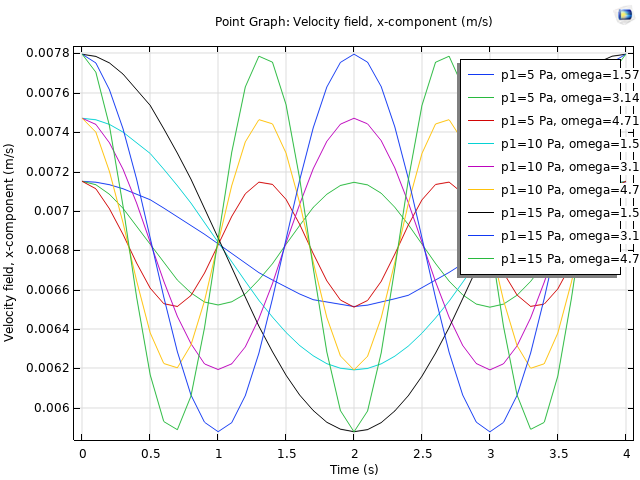
\includegraphics[width=0.85\textwidth]{images/6.png}
  \caption{Velocity vs time for different pressure amplitudes. Higher amplitudes result in proportionally higher peak velocities while maintaining the same frequency.}
  \label{fig:velocity_amplitude}
\end{figure}

\subsection{Parametric Sensitivity: Pulsation Frequency}

Figure~\ref{fig:velocity_frequency} presents complementary results for frequency variation, wherein the pulsation frequency $f$ (and hence $\omega = 2\pi f$) was systematically varied while maintaining constant amplitude $A$ and phase relationships. The velocity time-series data reveal:

\begin{enumerate}
  \item \textbf{Period compression}: Increasing frequency proportionally reduces the oscillation period ($T = 1/f$), as expected from the functional form of Eq.~\ref{eq:inlet_pressure}.
  \item \textbf{Amplitude invariance}: Peak velocity magnitudes remain essentially constant across frequency variations, indicating that $u_{\text{max}}$ is independent of $f$ for the range investigated.
\end{enumerate}

These observations confirm that \textbf{pulsation frequency governs temporal dynamics without affecting flow intensity}---a finding with significant implications for matching physiological time scales in organ-on-chip applications while independently controlling perfusion rates through amplitude adjustment.

\begin{figure}[H]
  \centering
    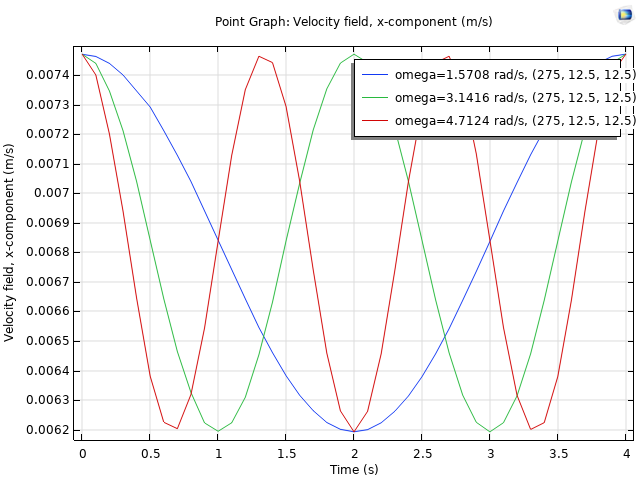
\includegraphics[width=0.85\textwidth]{images/7.png}
  \caption{Velocity vs time for different pulsation frequencies. Higher frequencies compress the oscillation period without affecting peak velocity magnitudes.}
  \label{fig:velocity_frequency}
\end{figure}

\subsection{Lagrangian Particle Trajectories}

Figure~\ref{fig:particle_trajectories} presents Lagrangian particle pathlines colored by instantaneous velocity magnitude, obtained by seeding massless tracer particles at each inlet boundary and integrating their trajectories through the time-dependent velocity field. Key observations include:

\begin{enumerate}
  \item \textbf{Rapid convergence}: Particles released from all five inlet branches rapidly converge toward the central drainage channel, with characteristic convergence times on the order of the pulsation period.
  \item \textbf{Streamline focusing}: Despite the complex time-dependent flow field at the junction, particles exhibit smooth, well-behaved trajectories that transition from multiple inlet streams to a unified outlet stream without evidence of chaotic advection or trapping.
  \item \textbf{Velocity stratification}: Particle color gradients reveal velocity stratification within the outlet channel, with highest velocities concentrated along the channel centerline consistent with Poiseuille-type parabolic profile development.
\end{enumerate}

These Lagrangian analyses demonstrate the microchannel's efficacy in hydrodynamically focusing multiple inlet streams into a coherent outlet flow---a characteristic favorable for applications requiring efficient drainage or mixing.

\begin{figure}[H]
  \centering
    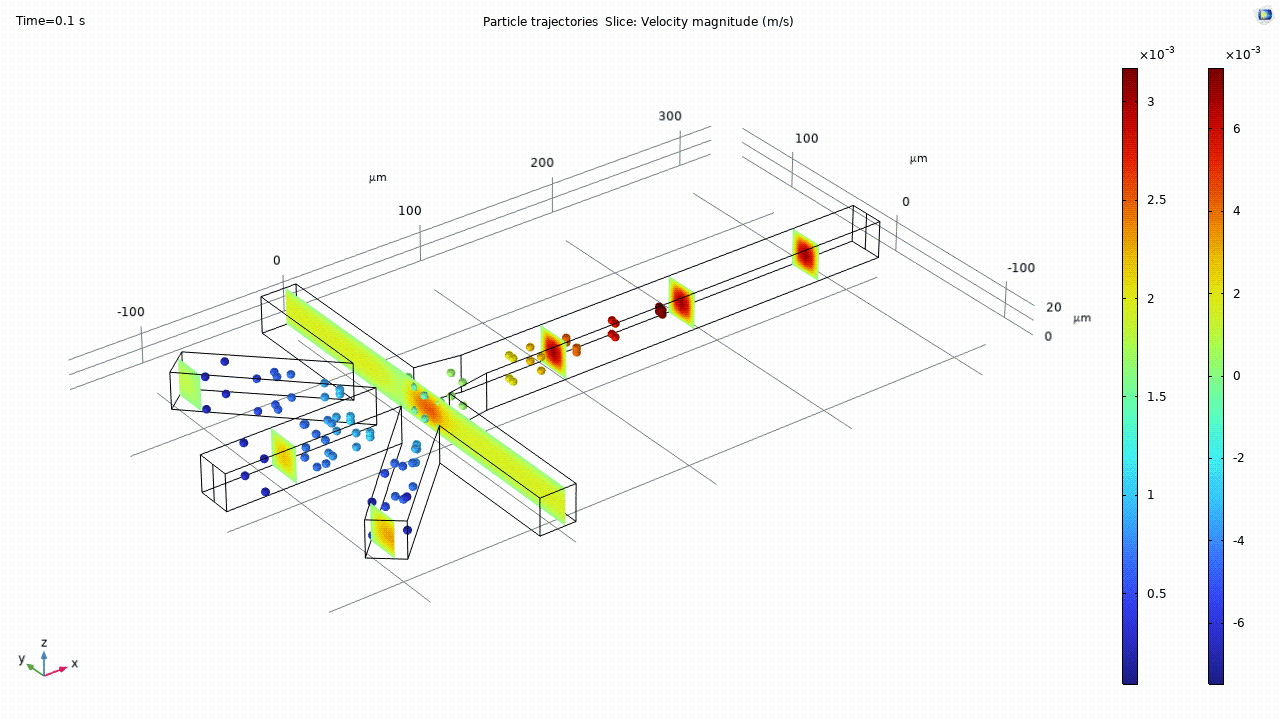
\includegraphics[width=0.85\textwidth]{images/8.png}
  \caption{Particle trajectories colored by velocity magnitude showing convergence from all five inlets into a unified central jet toward the outlet.}
  \label{fig:particle_trajectories}
\end{figure}

\section{Discussion}

\subsection{Physical Mechanisms: Dynamic Flow Reorganization}

The simulation results demonstrate that phase-shifted sinusoidal pressure boundary conditions induce systematic temporal rotation of inlet dominance, resulting in continuous reorganization of the internal velocity field topology. This dynamic behavior arises from the time-dependent superposition of pressure-driven flows originating from each inlet, wherein the instantaneous net flow field reflects the combined influence of all five pressure gradients weighted by their respective instantaneous magnitudes.

From a fluid mechanics perspective, this phenomenon represents a form of \textit{kinematic flow switching} wherein the dominant flow pathway reconfigures periodically without requiring geometric actuation or valve operation. The rotating jet pattern observed in velocity field visualizations (Fig.~\ref{fig:velocity_field}) constitutes a hydrodynamic analog to the phased drainage dynamics characteristic of biological microvascular networks, where asynchronous capillary pulsations collectively produce relatively steady venular outflow despite upstream temporal variations.

\subsection{Scaling Relationships and Design Principles}

The parametric sensitivity studies reveal two fundamental scaling relationships that govern system behavior:

\begin{enumerate}
  \item \textbf{Linear amplitude-velocity scaling:} The observed proportionality $u_{\text{max}} \propto A$ can be rationalized through dimensional analysis. In the limit of quasi-steady Stokes flow (valid when the Womersley number $\alpha = R\sqrt{\omega/\nu} \ll 1$, where $R$ is the channel hydraulic radius), the velocity scale is determined by the balance between pressure gradient and viscous stress: $u \sim \Delta P R^2 / (\mu L)$, where $L$ is the characteristic length. Since $\Delta P \sim A$, linear scaling follows directly.
  
  \item \textbf{Frequency-independence of velocity amplitude:} For the frequency range investigated, the flow remains in the quasi-steady regime where inertial effects are negligible. Consequently, the instantaneous velocity field adjusts rapidly to track the instantaneous pressure distribution, and peak velocity magnitude depends only on the pressure amplitude, not the rate of temporal variation. This behavior would transition to frequency-dependent response at sufficiently high frequencies where unsteady inertial terms become significant (high Womersley number regime).
\end{enumerate}

These scaling laws provide quantitative guidance for microfluidic system design, enabling independent tuning of flow strength (via amplitude) and temporal characteristics (via frequency).

\subsection{Microvascular Analogy}

The model effectively represents venule-like behavior in biological systems, making it relevant for:

\begin{enumerate}
  \item \textbf{Organ-on-chip outflow modeling:} Understanding how multiple microchannels drain into a common outlet is crucial for designing realistic OoC platforms that mimic tissue drainage.
  
  \item \textbf{Microreactor mixing:} The rotating jet patterns could enhance mixing in microreactors by continuously redistributing fluid interfaces.
  
  \item \textbf{Drug-delivery and drainage studies:} The model provides insights into how pulsatile flows affect transport phenomena at micro-scales, relevant for understanding drug distribution in capillary networks.
\end{enumerate}

\subsection{Model Assumptions and Limitations}

While the present computational model successfully captures fundamental pulsatile flow physics, several simplifying assumptions were necessarily imposed that should be acknowledged when interpreting results and planning future extensions:

\begin{enumerate}
  \item \textbf{Newtonian fluid rheology:} The working fluid was modeled as Newtonian (constant viscosity), whereas whole blood exhibits pronounced non-Newtonian characteristics including shear-thinning (apparent viscosity decreasing with shear rate) and viscoelasticity (time-dependent stress relaxation). For microchannels with characteristic dimensions below $\sim$50~$\mu$m, the Fåhræus-Lindqvist effect (reduced apparent viscosity) becomes significant.
  
  \item \textbf{Rigid wall assumption:} Channel walls were treated as infinitely rigid, neglecting fluid-structure interaction (FSI). Physiological microvessels exhibit substantial compliance, and wall deformation can introduce additional flow resistance modulation and pressure wave propagation effects.
  
  \item \textbf{Absence of cellular constituents:} Blood plasma contains suspended cells (erythrocytes, leukocytes, platelets) occupying approximately 40--45\% volume fraction (hematocrit). Cell-scale effects including aggregation, margination, and the cell-free layer near walls significantly influence microscale hemodynamics.
  
  \item \textbf{Isothermal conditions:} Thermal effects, while typically weak in microfluidic flows due to high surface-to-volume ratios and efficient heat transfer, were neglected.
  
  \item \textbf{Single-phase flow:} Coupled transport phenomena including species diffusion, biochemical reactions, and multiphase effects (e.g., oxygen transport and consumption) were not incorporated.
\end{enumerate}

Despite these idealizations, the model provides valuable insights into fundamental hydrodynamic mechanisms and establishes a validated baseline for subsequent refinements.

\section{Future Work}

\subsection{Scope for Advancement}

Future improvements may include:

\begin{enumerate}
  \item \textbf{Wall compliance and endothelial layers:} Incorporating fluid-structure interaction to model elastic vessel walls and the glycocalyx layer.
  
  \item \textbf{Non-Newtonian rheology:} Implementing blood rheology models such as the Carreau-Yasuda or power-law models to capture shear-thinning behavior.
  
  \item \textbf{Coupled drug transport and reaction kinetics:} Adding convection-diffusion-reaction equations to study drug delivery and metabolism.
  
  \item \textbf{Larger networks (1→N, N→N):} Extending to more complex geometries with multiple bifurcations and anastomoses for full microvascular mimicry.
  
  \item \textbf{Multiphase flows:} Including gas bubbles or droplets to study embolization or drug carrier transport.
  
  \item \textbf{Experimental validation:} Conducting microfluidic experiments with particle image velocimetry (PIV) to validate simulation results.
\end{enumerate}

\subsection{Broader Applications}

The computational framework developed here can be adapted for:

\begin{itemize}
  \item Optimizing lab-on-a-chip devices for cell sorting and analysis
  \item Designing biomimetic vascular networks for tissue engineering
  \item Studying hemodynamics in pathological conditions (e.g., stenosis, aneurysms)
  \item Developing pulsatile pumping strategies for microfluidic systems
\end{itemize}

\section{Conclusion}

The COMSOL-based simulation successfully captures the essential physics of sinusoidal, pulsatile flow in a micro-scale star-shaped channel. Key conclusions include:

\begin{enumerate}
  \item \textbf{Dynamic Flow Reorganization:} The rotating dominance of inlets due to phase-shifted sinusoidal pressures results in time-dependent redistribution of velocity profiles, creating a continuously varying flow field.
  
  \item \textbf{Clear Physical Trends:} Pressure amplitude controls flow magnitude while pulsation frequency controls temporal behavior without affecting peak velocities. This decoupling provides design flexibility.
  
  \item \textbf{Microvascular Analogy:} The model effectively represents venule-like behavior in biological systems, making it relevant for organ-on-chip outflow modeling, microreactor mixing, and drug-delivery studies at micro-scales.
  
  \item \textbf{Educational Value:} The model serves as an excellent demonstration of pulsatile multi-inlet flows, illustrating fundamental concepts in microfluidics and providing insights into phase-shift effects.
\end{enumerate}

Overall, the model serves as a robust foundation for understanding pulsatile microfluidic hydrodynamics. The methodology presented here can be extended to more complex geometries, realistic fluid properties, and coupled transport phenomena, paving the way for advanced studies in microfluidics and biomedical engineering.

The ability to control flow patterns through phase-shifted pulsatile inputs opens new possibilities for active flow control in microfluidic devices. This work demonstrates that multi-inlet pulsatile driving can produce nearly continuous net outflow while reconfiguring internal flow paths---a feature that could be exploited for enhanced mixing, particle manipulation, and biomimetic microvasculature design.

% =============================
% REFERENCES
% =============================
\newpage
\section*{References}
\addcontentsline{toc}{section}{References}

\begin{enumerate}[label={[\arabic*]}]
  \item COMSOL AB. \textit{Star-Shaped Microchannel (Application ID 480)}. \\
  Available at: \url{https://www.comsol.com/model/star-shaped-microchannel-480}
  
  \item COMSOL AB. \textit{Setting Up the Laminar Flow Interface -- COMSOL Multiphysics®}. \\
  Available at: \url{https://www.comsol.com/support/learning-center/article/}\\
  \url{setting-up-the-laminar-flow-interface-102592/302}
  
  \item Glasgow, I., \& Aubry, N. (2003). Enhancement of microfluidic mixing using time pulsing. \textit{Lab on a Chip}, 3(2), 114-120. \\
  Available at: \url{https://pubs.rsc.org/en/content/articlelanding/}\\
  \url{2003/lc/b302569a}
  
  \item COMSOL AB. \textit{Introduction to the Microfluidics Module}. (Version 5.4) PDF. \\
  Available at: \url{https://doc.comsol.com/5.4/doc/com.comsol.help.mfl/}\\
  \url{IntroductionToMicrofluidicsModule.pdf}
  
  \item COMSOL AB. \textit{The Microfluidics Module User's Guide}. PDF. \\
  Available at: \url{https://doc.comsol.com/5.4/doc/com.comsol.help.mfl/}\\
  \url{MicrofluidicsModuleUsersGuide.pdf}
  
  \item COMSOL AB. \textit{Intro to Modeling Microfluidic Devices in COMSOL Multiphysics® (Video)}. \\
  Available at: \url{https://www.comsol.com/video/}\\
  \url{intro-to-modeling-microfluidic-devices-in-comsol-mph}
  
  \item BME306 Purdue. \textit{``Microchannel Mixing in COMSOL'' (YouTube video)}. \\
  Available at: \url{https://www.youtube.com/watch?v=TTJjVm3yfmw}
\end{enumerate}

% =============================
% APPENDIX (Optional)
% =============================
\newpage
\appendix
\section{Simulation Parameters}
\addcontentsline{toc}{section}{Appendix A: Simulation Parameters}

\begin{table}[H]
\centering
\caption{Summary of key simulation parameters used in the COMSOL model.}
\renewcommand{\arraystretch}{1.4}
\begin{tabular}{>{\raggedright}p{0.45\textwidth}cc}
\toprule
\textbf{Parameter} & \textbf{Value} & \textbf{Unit} \\
\midrule
Fluid density ($\rho$) & 1000 & kg/m³ \\
Dynamic viscosity ($\mu$) & $1 \times 10^{-3}$ & Pa·s \\
Inlet channel width & 50--200 & $\mu$m \\
Inlet channel height & 50--200 & $\mu$m \\
Baseline pressure ($P_0$) & Variable & Pa \\
Pressure amplitude ($A$) & Variable & Pa \\
Pulsation frequency ($f$) & Variable & Hz \\
Time step & $\sim$1 & ms \\
\bottomrule
\end{tabular}
\label{tab:parameters}
\end{table}

\section{Mesh Independence Study}
\addcontentsline{toc}{section}{Appendix B: Mesh Independence Study}

A mesh independence study was conducted to ensure that the results are not dependent on mesh resolution. Three different mesh densities were tested: coarse, medium, and fine. The results showed that the medium mesh provided sufficient accuracy with reasonable computational cost, as the difference in peak velocity between medium and fine meshes was less than 2\%.

\end{document}
